\documentclass[a4paper]{proc}

\usepackage{amsfonts}
\usepackage{amsmath}
\usepackage{oz}
\usepackage{algorithm}
\usepackage{algpseudocode}
\usepackage{graphicx}

\newcommand{\Break}{\State \textbf{break}}

\title{Rex Ready: A TAC Classic agent implementation}
\author{James Robinson\thanks{COMP6203 Group 10: Peter Prince, James Robinson, Andrew Sullivan}}

\begin{document}

\maketitle

\begin{abstract}
  In this paper I describe our TAC Classic agent, \emph{Rex Ready}, which achieved a second place finish in the 2014 COMP6203 class tournament. \emph{Rex Ready} relies on \emph{Bayesian updating} and \emph{fuzzy logic} to build a model of predicted market prices, and a \emph{hill-climbing optimiser} to select the optimum bidding strategy taking into account client preferences, predicted market prices, and availability data.
\end{abstract}

\section{Introduction}

Rex Ready is a TAC Classic agent implemented in Java. Due to space constraints, the TAC Classic ruleset will not be described in detail in this paper.

Rex Ready consists of three main components:

\begin{itemize}
  \item A price prediction module, which attempts to predict:
  \begin{itemize}
    \item The minimum price that each flight ticket will reach between the current time and the end of the game, and
    \item The closing price of each hotel auction, under the assumption that they will all close at the end of the current minute,
  \end{itemize}
  \item An optimiser, which attempts to find a strategy that maximises the agent's score, and
  \item A bidding component, which invokes the optimiser to select a strategy, and uses that strategy to place bids.
\end{itemize}

\section{Price prediction}

\subsection{Flight price prediction}

\subsection{Hotel price prediction}

\subsection{Entertainment price prediction}

\section{Optimisation}

\begin{algorithm}
  \caption{Optimisation}
  \label{alg:optimisation}
  \begin{algorithmic}
    \small
    \State $CurrentStrategy \gets \Call{InitialStrategy}{}$

    \Function{Optimise}{$Timeout$}
      \State $StartTime \gets \Call{CurrentTime}{}$

      \While{$\Call{CurrentTime}{} < StartTime + Timeout$}
        \State $NewStrategy \gets CurrentStrategy$
        \For{10 iterations}
          \State $NewStrategy \gets \Call{Mutate}{NewStrategy}$
          \If{$\Call{Score}{NewStrategy} > \Call{Score}{CurrentStrategy}$}
            \State $CurrentStrategy \gets NewStrategy$
            \Break
          \EndIf
        \EndFor
      \EndWhile
      \State \Return{CurrentStrategy}
    \EndFunction
  \end{algorithmic}
\end{algorithm}

Our agent's optimiser is implemented as a hill climber. Upon initialisation, the optimiser selects an initial strategy by simply constructing packages for each client matching their preferences. This strategy is rarely optimal, put provides a good starting point for successive improvement.

Pseudocode for the optimiser is given in algorithm~\ref{alg:optimisation}. The \texttt{Optimise} function completes as many generations as it can before the timeout elapses. During each generation the current best strategy is mutated, and if the result has a higher score then it replaces the previous best. In order to prevent the optimiser from becoming stuck at local optima, it is allowed to perform up to 10 successive mutations per generation.

The score function obtains a list of goods that will need to be purchased in order to complete a given strategy, calculates the total cost of those goods, and subtracts that from the sum of the utility values for all the packages within the strategy.

A strategy is \emph{feasible} if all of the goods it requires are available. If a strategy is infeasible, a penalty of 10000 is applied to its score (simply awarding a score of 0 to any infeasible package creates ``cliffs'' in the objective function, which makes it very difficult for the optimiser to find the global maximum).

The mutation operator for a strategy has a chance to remove or replace packages within the strategy. This allows the optimiser to consider strategies that do not provide packages for all 8 clients.

The use of an optimiser (as opposed to bidding solely based on heuristics) makes the agent robust against other agents bidding illogically, unfortunate hotel closures, etc. It also allows the agent to consider the benefits of forgoing the utility bonuses that come from obeying client preferences in favour of reducing costs.

\subsection{Mutation rate}

\begin{figure}
  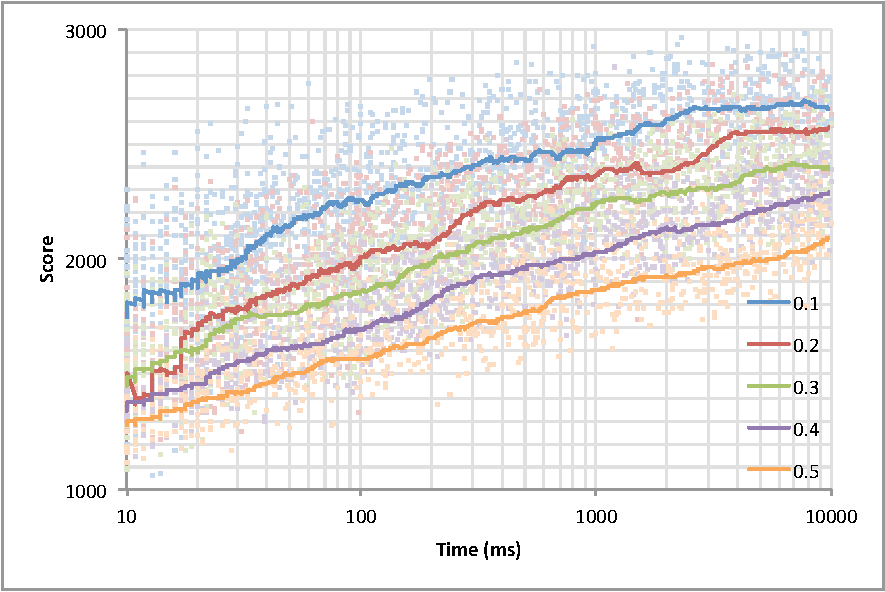
\includegraphics[width=\linewidth]{mutation_rate_1.pdf}
  \caption{Time vs score for mutation rates in interval [0.1, 0.5]}
  \label{fig:mutation_rate_1}
\end{figure}

\begin{figure}
  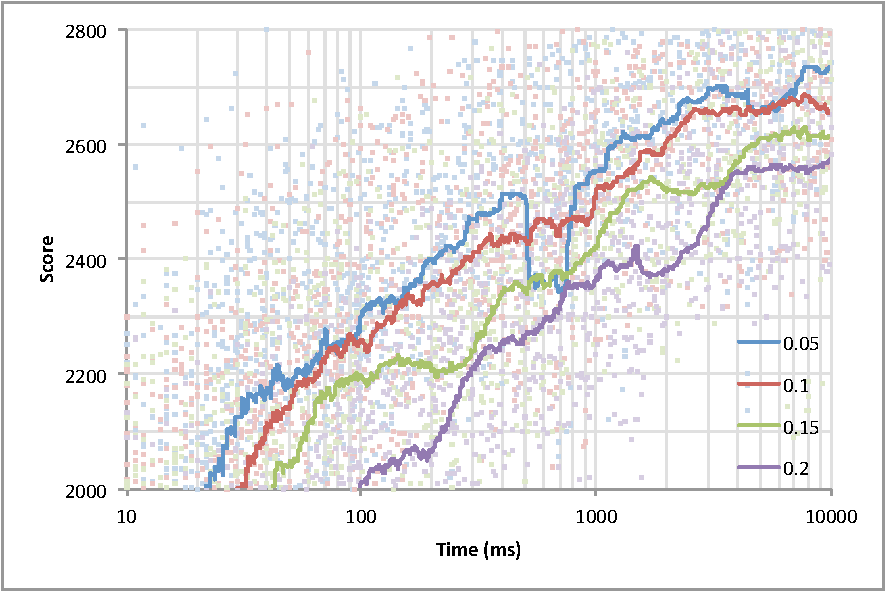
\includegraphics[width=\linewidth]{mutation_rate_2.pdf}
  \caption{Time vs score for mutation rates in interval [0.05, 0.2]}
  \label{fig:mutation_rate_2}
\end{figure}

\begin{figure}
  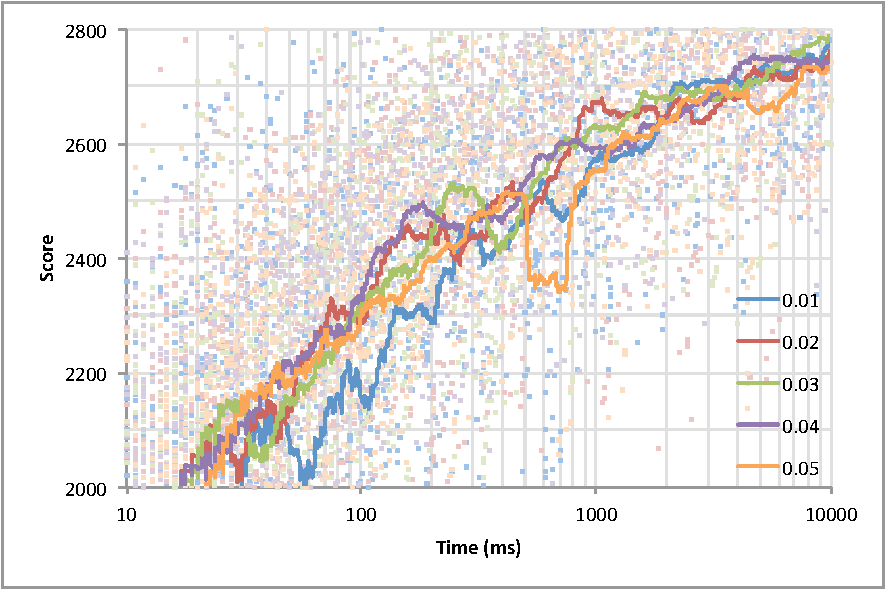
\includegraphics[width=\linewidth]{mutation_rate_3.pdf}
  \caption{Time vs score for mutation rates in interval [0.01, 0.05]}
  \label{fig:mutation_rate_3}
\end{figure}

Chosing a suitable mutation rate was critical to the performance of the agent, since the optimiser is only provided with a limited amount of time in which to find an optimal solution. In order to select a good mutation rate, the current predicted prices, availability, and owned goods were captured during a game in order to set up a realistic scenario in which to test the optimiser in isolation, and the optimiser was allowed to run for 10 seconds with various different mutation rates. Each mutation rate was tested 100 times in an attempt to smooth out random variations in performance.

Figure~\ref{fig:mutation_rate_1} shows mutation rates in the interval [0.1, 0.5] in steps of 0.1. A mutation rate of 0.1 proved most effective in this test, reaching its highest score significantly faster than any other rate.

Mutation rates in the interval [0.05, 0.2] in steps of 0.05 were then tested, and the results are shown in figure~\ref{fig:mutation_rate_2}. The optimal mutation rate in this second test was 0.05.

A third and final test was performed with mutation rates in the interval [0.01, 0.1] in steps of 0.01 (illustrated in figure~\ref{fig:mutation_rate_3}), but the results were too noisy to draw any statistically significant conclusions.

Based on these experiments, a mutation rate of 0.05 was selected for the optimiser.

\section{Bidding strategy}

At the very start of each game, the agent immediately attempts to gain inventory by placing bids for 8 of each hotel room at a price of 10 each, and 1 of each type of entertainment at a price of 50 each. The agent does not perform any informed bidding for the first 30 seconds of the game, in order to allow the prices to settle and the price predictors to begin producing sensible estimates.

Depending on the competitiveness of the hotel bidding environment, the optimiser might not settle on a strategy until very late in the game. For this reason, the agent is forbidden from placing any bids on flights or entertainment until the 4th minute, after the first 3 hotel auctions close. This prevents the agent from purchasing expensive flight tickets that it will not need, and also prevents it from selling entertainment tickets that it may need in the future.

Bidding is performed on ``bid ticks'', which occur each time the last flight action's quote is updated (every 10 seconds). During a bid tick the agent updates its price estimates and runs the optimiser for a fixed duration (7 seconds) in order to pick the bidding strategy for that tick. Once a new strategy has been determined, the agent clears and replaces its allocations based on the requirements of the selected strategy. If the score projection provided by the optimiser is positive, then the agent will proceed to place bids as detailed below. If the score projection is zero or negative, the agent will skip the current bid tick in the hope that the optimiser will find a profitable strategy in a future bid tick.

\subsection{Flight bidding}

In order to minimise costs, the agent attempts to purchase flights at their predicted minimum price rather than at a specific time. During each bid tick after the 4th minute, the agent will purchase required flight tickets if:

\begin{itemize}
  \item The ticket's current ask price is within 10 of its projected minimum, or
  \item There are less than 30 seconds of the game remaining.
\end{itemize}

\subsection{Entertainment bidding}

During each bid tick after the 4th minute, the agent will:

\begin{itemize}
  \item Place buy bids for required entertainment tickets at the current ask price, or 200, whichever is lower
  \item Place sell bids for all owned but not required entertainment tickets at the current ask price - 10, or 60, whichever is higher
\end{itemize}

During the practice games, a previous revision of our agent placed a bid for an alligator wrestling ticket for a price of over 9000 by mistake. In order to prevent this from happening again, we added a restriction that the agent will never bid more than 200 (the maximum possible utility bonus entertainment can provide) for each ticket, in addition to the restriction that the agent cannot bid when the projected score provided by the optimiser is below 0.

Entertainment tickets are never sold for less than 60 because the utility bonus that the purchaser would gain from the ticket is likely to be greater than the amount of profit our agent would make from the transaction, meaning that the transaction is likely to hurt our agent's position in the tournament rankings.

In addition, the agent will attempt to sell entertainment tickets that it does not need \emph{or even own} for at least 200, since this amount is equal to the oversell penalty. In practice, very few agents purchase tickets for above 200 since such tickets provide no utility bonus, but this rule allows us to take advantage of poorly-designed or malfunctioning agents to improve our ranking.

\subsection{Hotel bidding}

During the final bid tick of each minute, the agent places hotel bids in the following manner for each hotel auction:

\begin{itemize}
  \item Let $HQW$ (\emph{hypothetical quantity won}) be the number of rooms the agent would have bought if the auction had closed at the end of the previous minute
  \item Let $alloc$ be the number of rooms that we need
  \item Place a bid for $alloc$ rooms at the predicted price + 50
  \item If $alloc < HQW$, place a bid for $HQW - alloc$ hotel rooms at the current ask price + 1
\end{itemize}

By placing the lowest allowed bid for goods that the agent no longer needs, we maximise the possibility that another agent will purchase those goods, meaning we do not have to pay for them.

\section{Performance}

During the practice games, our agent was run under the pseudonym ``ComeOnAndSlam''. Under this guise, Rex Ready managed to top the leaderboard with a mean score of 3251.56 across its nonzero games.

During the tournament itself our agent fared similarly well, finishing in second place with an overall score of 3099.58 - just 210 points behind the leader, and more than 400 points ahead of the agent that finished in third place.

Our agent was able to deal very well with poorly performing or malfunctioning agents, as well as games with highly competitive markets for hotel rooms, by considering every possible strategy rather than relying on simple heuristics.

The flight price predictions proved to be surprisingly accurate (considering the prices follow a random walk), making it possible for the agent to obtain flight tickets for the cheapest possible amount. The hotel price predictions, although far less accurate than the flight predictions (perhaps due to the differences in bidding strategies between the agents in each game), proved sufficient to allow the optimiser to select strategies effectively.

Attempting to predict the minimum price of entertainment tickets proved futile, because:

\begin{itemize}
  \item The agents in the competition had a very wide spread of entertainment bidding strategies, making it very difficult to predict prices from historical data, and
  \item Although many agents paid sensible amounts for entertainment, a few always chose to bid at the current ask price (even if that price was above 200).
\end{itemize}

We therefore opted to simply use the current ask prices during the optimisation stage, instead of attempting to predict future prices. The agent was able to perform well in spite of this limitation.

\subsection{Score analysis}

\begin{table}
  \caption{Table of scores}
  \label{tab:scores}
  \center
  \begin{tabular}{ c | r r r }
    Game & Utility & Cost    & Score   \\
    \hline
    614  & 5845    & 2785.96 & 3059.04 \\
    617  & 8755    & 4070.32 & 4684.68 \\
    618  & 10315   & 6438.42 & 3876.58 \\
    622  & 10180   & 7278.55 & 2901.45 \\
    624  & 8732    & 4295.10 & 4436.90 \\
    630  & 7925    & 5806.98 & 2118.02 \\
    631  & 7892    & 5085.70 & 2806.30 \\
    634  & 8150    & 5429.91 & 2720.09 \\
    639  & 8580    & 6312.76 & 2267.24 \\
    640  & 8416    & 6766.44 & 1649.56 \\
    641  & 7998    & 4285.68 & 3712.32 \\
    645  & 8943    & 6816.13 & 2126.87 \\
    647  & 7685    & 5170.85 & 2514.15 \\
    652  & 8605    & 4388.50 & 4216.50 \\
    654  & 9030    & 5348.05 & 3681.95 \\
    655  & 8343    & 5521.44 & 2821.56 \\
    \hline
    Mean & 8462.13 & 5362.55 & 3099.58 \\
    IQM  & 8447.38 & 5383.02 & 3027.11 \\
    SD   & 1017.41 & 1203.13 &  904.17 \\
  \end{tabular}
\end{table}

Table~\ref{tab:scores} shows the utility, cost, and overall score the agent achieved in each game it participated in. The mean, interquartile mean (\emph{IQM}) and standard deviation (\emph{SD}) are shown for each variable.

As there are no obvious outliers in the dataset, the mean and IQM match fairly closely. The lower IQM of the score relative to the mean might be attributed to the fact 4 of the opposing agents in game 617 malfunctioned, artificially lowering the hotel and entertainment prices for that game and thereby inflating our score - the IQM does not include this game.

The standard deviation for overall score is far lower than that of utility and cost due to the fact that the optimiser considers every possible strategy rather than simply choosing to minimise cost or maximise utility.

\end{document}
